{\fontsize{12pt}{22pt} \textbf{K-means}\par}

\vspace{5mm}

(see kmeans.pdf from OneDrive folders for more details)

\vspace{5mm}

Objective: group data into $k$ clusters so that samples in the same cluster are close to each other w.r.t. the Euclidean distance.

\vspace{5mm}
The cost function minimization is written as such:

$$\underset{C_1,...,C_k;\mu_1,...,\mu_k}{\operatorname{argmin}}\Sigma_{j=1}^k\Sigma_{i \in C_j}||x_i-\mu_j||^2$$

Where $\mu_j$ is the mean, also called gravity center or cluster center:

$$\mu_j=\frac{1}{|C_j|}\Sigma_{i \in C_j}x_i$$

\begin{algorithm}
\caption{K-means}
\begin{algorithmic}
\State Input: $x_1,...,x_n$
\State Output: clusters $C_1,...,C_k$
\State Random values for $\mu_1,...,\mu_k$
\While{no convergence}
\State // Step 1: Update clusters
\State $C_1,...,C_k \leftarrow \emptyset$
\For{$i=1$ to $n$}
\State $j \leftarrow argmin_l ||x_i - \mu_l||$
\State $C_j \leftarrow C_j + \{i\}$ // We add observation $i$ to the cluster $C_j$
\EndFor
\State // Step 2: Update cluster centers
\For{$j=1$ to $k$}
\State $\mu_j \leftarrow 0$
\State $n_j \leftarrow 0$
\For{$i$ in $C_j$} // We loop on all observations of each cluster
\State $\mu_j \leftarrow \mu_j + x_i$
\State $n_j \leftarrow n_j +1$
\EndFor
\State $\mu_j \leftarrow \mu_j /n_j$
\EndFor
\EndWhile
\end{algorithmic}
\end{algorithm}

The quality of the clustering strongly depends on the initial center values. This is why the algorithm is generally run multiple times for different initial values. The best clustering (i.e., that of minimum cost) is returned.

\vspace{5mm}

\underline{K-means++}

To improve the quality of the clustering, we choose the initial cluster centers far from each other:

- select the first cluster center uniformly at random among the n data samples

- select the following cluster centers at random, with a probability proportional to the square distance to the closest current cluster center

\lstset{language=Python}
\lstset{frame=lines}
\lstset{caption={K-means++ initial centers selection}}
\lstset{label={lst:code_direct}}
\lstset{basicstyle=\footnotesize}
\begin{lstlisting}

centers = []
centers.append(X[np.random.randint(X.shape[0])]) # inital center = one random sample
distance = np.full(X.shape[0], np.inf) # a vector (n,1) with only infinity terms
for j in range(1,self.n_clusters):
    distance = np.minimum(np.linalg.norm(X - centers[-1], axis=1), distance) # size (n,1); 
# distance = the smallest distance associated with 
# the last added center
    p = np.square(distance) / np.sum(np.square(distance)) # probability vector [p1,...,pn]
# the highest probability in p is associated 
# with the biggest distance w.r.t the last added center
    sample = np.random.choice(X.shape[0], p = p) # one sample is 
						 # selected according to probabilities
    centers.append(X[sample])

\end{lstlisting}

\textcolor{gray}{Note: this problem is called \textit{NP-hard problem}. It means that its complexity is at least equal to the complexity of an NP-problem}

\textcolor{gray}{NP-problem: a problem is NP if it can be determined by a non-deterministic Turing machine in polynomial time. Intuitively, a problem is NP if we can quickly verify if one candidate is a solution of the problem. E.g. "travelling salesman problem" = let $d$ be a distance and $n$ be a number of cities. Is there an itinerary with distance $\ge d$ stopping by every city? -> easy to check...}

\vspace{5mm}
\textcolor{gray}{Turing machine (1936)}

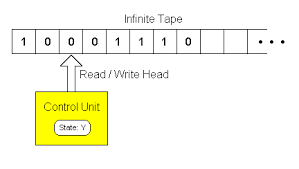
\includegraphics{../images/turingmachine.png}

\textcolor{gray}{"non-deterministic turing machine": itinerary can be represented by a tree...}

\vspace{5mm}

